\documentclass[tikz, border=0pt]{standalone}
\usepackage[svgnames]{xcolor} 
\usepackage{tikz}
\usetikzlibrary{arrows.meta, shadows} 

\begin{document}
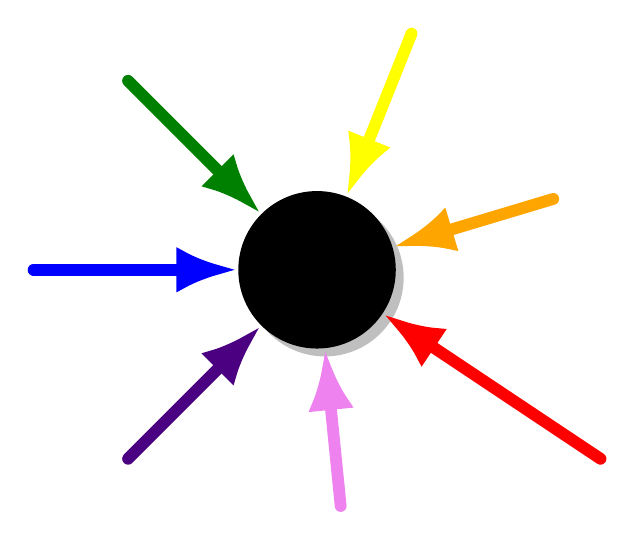
\begin{tikzpicture}[
    >=Latex,
    line cap=round,
    line join=round
]

\node[circle, fill=black, minimum size=2cm, drop shadow={shadow xshift=0.1cm, shadow yshift=-0.1cm, opacity=0.5}] (center) at (0,0) {};

\def\arrowlen{3cm}
\def\arrowwidth{1.5mm}

\draw[line width=\arrowwidth, fill=Red, color=Red, ->] (\arrowlen*1.2, -\arrowlen*0.8) -- (center);
\draw[line width=\arrowwidth, fill=Orange, color=Orange, ->] (\arrowlen, \arrowlen*0.3) -- (center);
\draw[line width=\arrowwidth, fill=Yellow, color=Yellow, ->] (\arrowlen*0.4, \arrowlen) -- (center);
\draw[line width=\arrowwidth, fill=Green, color=Green, ->] (-\arrowlen*0.8, \arrowlen*0.8) -- (center);
\draw[line width=\arrowwidth, fill=Blue, color=Blue, ->] (-\arrowlen*1.2, 0) -- (center);
\draw[line width=\arrowwidth, fill=Indigo, color=Indigo, ->] (-\arrowlen*0.8, -\arrowlen*0.8) -- (center);
\draw[line width=\arrowwidth, fill=Violet, color=Violet, ->] (\arrowlen*0.1, -\arrowlen*1) -- (center);

\end{tikzpicture}
\end{document}